%%This is a very basic article template.
%%There is just one section and two subsections.
\documentclass[a4paper, ngerman]{scrartcl}

\usepackage[T1]{fontenc}
\usepackage[utf8]{inputenc}
\usepackage[ngerman]{babel}
\usepackage{lmodern}
\usepackage{amsmath}
\usepackage{amsfonts}
\usepackage{hyperref}
\usepackage{graphicx}
\usepackage{paralist}
\usepackage[none]{hyphenat}

\sloppy



\hypersetup{ 
pdfborder = {0 0 0}, 
urlbordercolor = {0 0 0},
colorlinks = true,
linkcolor = black,
citecolor = black,
filecolor = black,
urlcolor  = black
}

\title{Software-Challenge 2015 - Hey,danke für den Fisch}
\subtitle{Spielregeln}



%% Variablen
\newcommand{\FelderAnzahl}{\emph{60}}
%%\newcommand{\KartenAnzahl}{\emph{KartenAnzahl}}
\newcommand{\PinguinAnzahl}{\emph{4}}
\newcommand{\EmptyPlainPage}{\newpage\thispagestyle{plain}\ \newpage}
\newcommand{\RundenAnzahl}{\emph{56}}

\begin{document}
\parindent0px
\maketitle

\begin{figure}[h!]
	\centering
	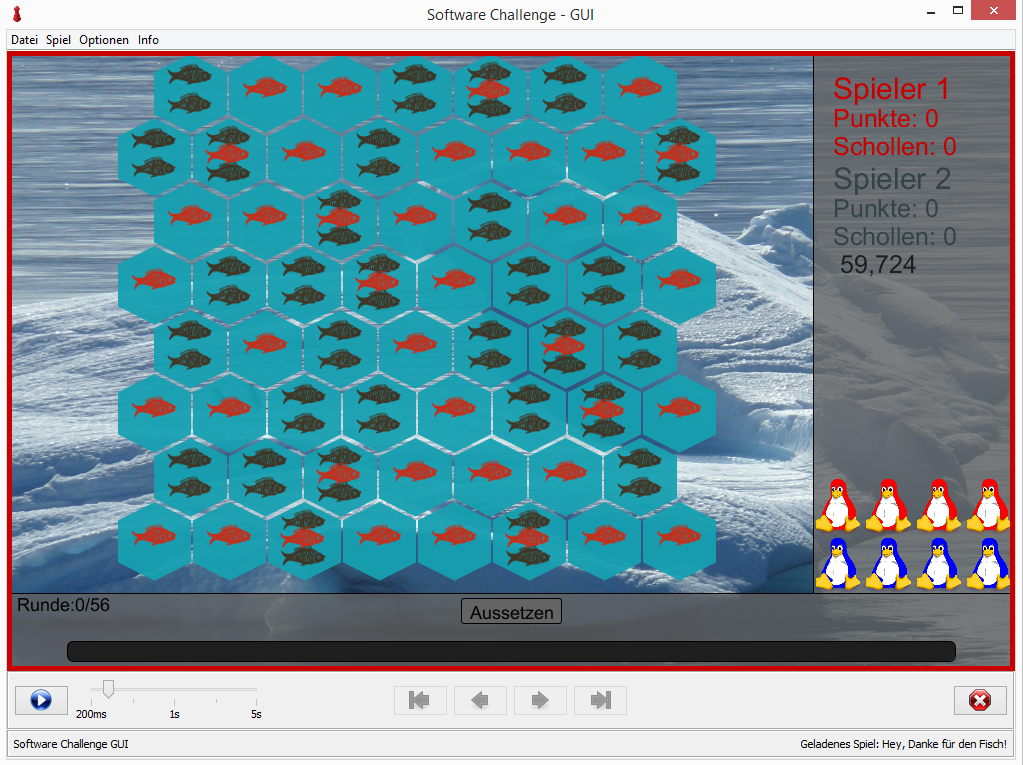
\includegraphics[width=\linewidth]{bilder/gui.png} 
\end{figure}
\vspace*{\fill}
"Die Nutzung des Spielkonzeptes "Hey, danke für den Fisch" (Name, Spielregeln
und Grafik) erfolgt mit freundlicher Genehmigung des Heidelberger
Spieleverlags."
\newpage
\tableofcontents
\newpage

\section{Einführung}
In dieser Anleitung werden die Elemente und Regeln des Spiels \emph{Hey,danke
für den Fisch} der Software-Challenge 2015 erläutert.\\
In dem Spiel versuchen zwei Spieler,
abwechselnd einen ihrer Pinguine zu bewegen und so Fische einzusammeln. Wer
am Ende des Spiels mehr Fische hat gewinnt das Spiel. Bei einem Gleichstand 
entscheidet die Anzahl der eingesammelten Eisschollen.\\
In der implementierten Version setzt jeder Spieler zuerst abwechselnd seine 
\PinguinAnzahl\ Pinguine auf Eisschollen mit nur einem Fisch und zieht dann
abwechselnd, beginnend mit dem Spieler der den letzten Pinguin gesetzt hat, seine Pinguine
über das Feld.

\section{Spielmaterial}
	\subsection{Das Spielbrett}
Das Spielbrett setzt sich aus \FelderAnzahl\ sechseckigen Eisschollen zusammen,
mit jeweils einem, zwei oder drei Fischen.
Die Verteilung der 30 Eisschollen mit einem Fisch, 20 mit zweien und 10 mit
dreien ist zufällig.
Jede gerade Reihe hat hierbei jeweils 7 Eisschollen und jede ungerade 8
Eisschollen, wobei die Zählung mit Null beginnt. Ein mögliches Spielbrett ist
in Abbildung~\ref{fig:Spielfeld} zu sehen.
\section{Spielablauf}	 

	%% an Beispiel erklären
	Es beginnt der rote Spieler. Jeder Spieler darf abwechselnd einen
	Zug machen. Innerhalb der ersten 4 Runden sind nur Setzzüge möglich. Ab der
	5.
	Runde sind beginnend mit dem blauen Spieler nur noch Laufzüge möglich.\\
	Sobald ein Spieler eine Figur ausgewählt hat, werden sämtliche Felder, auf
	welche die Figur ziehen kann, grün markiert.
	
	
	
	\subsection{Setzzüge}
	
	\begin{figure}[h!]
		\centering
		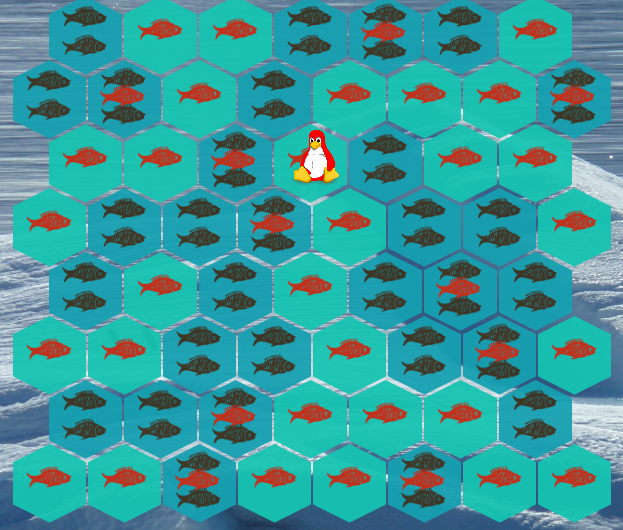
\includegraphics[scale = 0.4]{bilder/setzzug.png}
		\caption{Spielsituation in der Setzphase.}
		\label{fig:Setzzug}
	\end{figure}
	%% an Beispiel erklären
	Bei einem Setzzug wählt ein Spieler einen seiner
	Pinguine und setzt ihn auf eine Eisscholle ohne Pinguin, auf der sich nur ein
	Fisch befindet.\\
	Bei einem Setzzug kann nicht ausgesetzt werden. Durch klicken auf die
	jeweiilige Eisscholle wird der Pinguin gesetzt. 
	
	
	 
\subsection{Laufzüge}
	 
	\begin{figure}[h!]
		\centering
		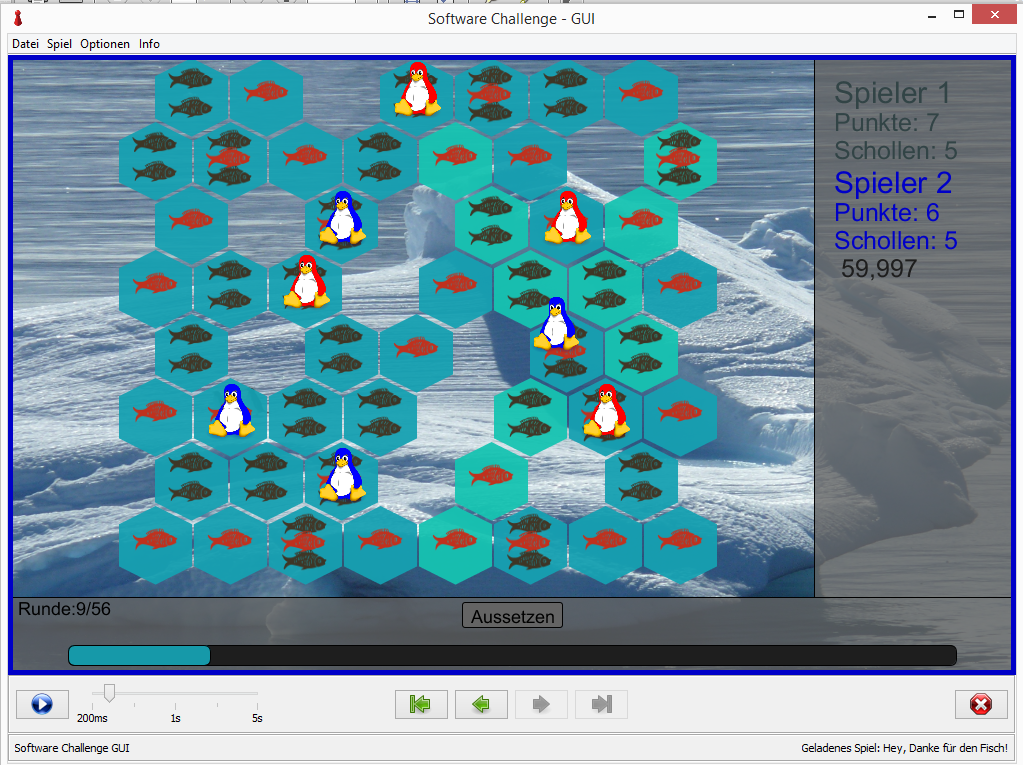
\includegraphics[scale=0.4]{bilder/laufzug.png}
		\caption{Eine Spielsituation in der Laufzugphase.}
		\label{fig:Laufzug}
	\end{figure}
	
%% an Beispiel erklären
Ab dem 9. Zug (anfang der 5. Runde) sind Laufzüge möglich. Bei einem Laufzug
ist es möglich einen Pinguin entlang der Horizantalen oder der beiden Diagonalen
zu bewegen. Ein Pinguin kann hierbei nicht über oder auf andere Pinguine oder
Löcher ziehen. Dabei wird die Fischanzahl des Feldes, auf dem sich der Pinguin
befunden hat dem Punktekonto hinzugefügt und die Anzahl der eingesammelten 
Eisschollen um 1 erhöht. Diese Eisscholle verschwindet daraufhin vom Spielfeld.



\subsection{Aussetzzüge}
%% an Beispiel erklären 
Ein Aussetzzug ist an Stelle eines Laufzugs möglich. Anstatt einen Pinguin zu 
setzten wird stattdessen nichts getan. Ein Aussetzzug ist normalerweise nur dann
sinnvoll, wenn kein anderer Zug mehr möglich ist.
	
\subsection{Punkteverteilung}
Die Punkte ergeben sich aus den eingesammelten Fischen. Bei einem Unendschieden
wird der Sieger nach der Anzahl der Eisschollen ermittelt.

	
\section{Ende des Spiels} 
	Können keine Spieler mehr Züge (ausgenommen Aussetzzüge) machen endet das
	Spiel und alle Felder auf denen noch ein Pinguin steht werden zu den Punkten
	hinzugefügt und die Eisschollenanzahl wird pro Pinguin um 1 erhöht. Es
	gewinnt der Spieler, der am meisten Fische hat oder falls die Anzahl gleich ist,
	wer mehr Eisschollen eingesammelt hat.
	Geschiet dies nicht innerhalb der \RundenAnzahl\ Runden,endet das Spiel
	ebenfalls.
	
\section{Die graphische Benutzeroberfläche}
\subsection{Übersicht der graphischen Benutzeroberfläche}
	In Abbildung~\ref{fig:GUI} ist ein Überblick der graphischen Benutzeroberfläche
	zu sehen. Die markanten Spielelemente sind mit \emph{a-e} gekennzeichnet.
	
	 \begin{figure}[h!]
		\centering		
		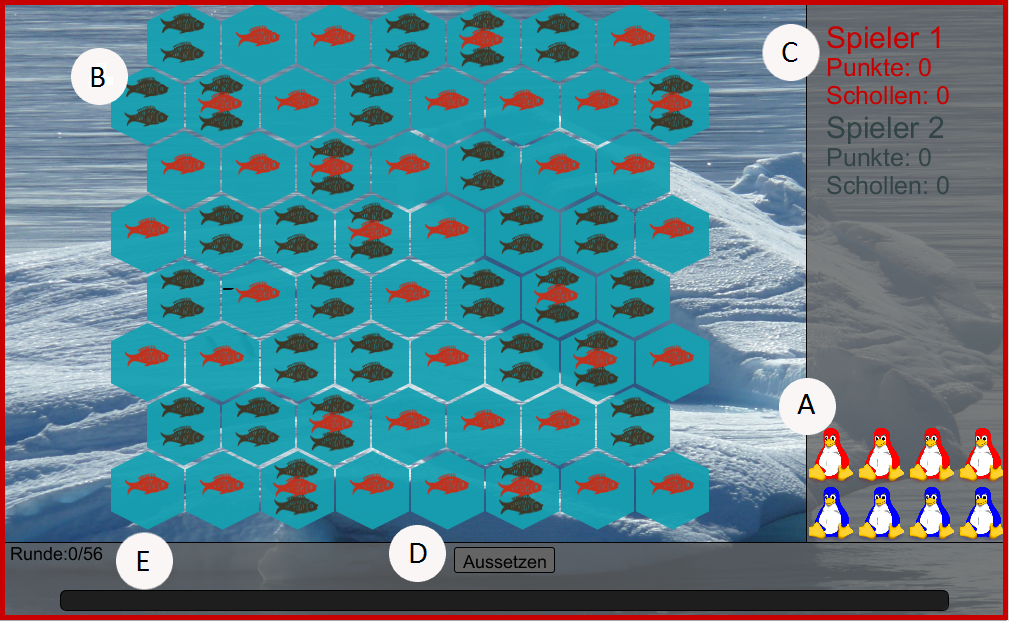
\includegraphics[scale = 0.5]{bilder/uebersicht.png} 
		\caption{Überblick der GUI}
		\label{fig:GUI}
	\end{figure} 
	%% wie ist die Benutzeroberfläche?
\begin{compactenum}[a)] \item Die Pinguine befinden sich anfangs links.
\item Das Spielbrett \item Punkteanzeige.
 Die Punkte des roten Spielers und Schollen sind 
oben, die des blauen Spielers unten. Die Punkte des inaktiven Spielers sind
jeweils immer grau.
\item Der Aussetzbutton
\item  Die Spielfortschrittsanzeige
	\end{compactenum}
	
\subsection{Das Einstellungsmenü} 
	 \begin{figure}[h!]
		\centering
		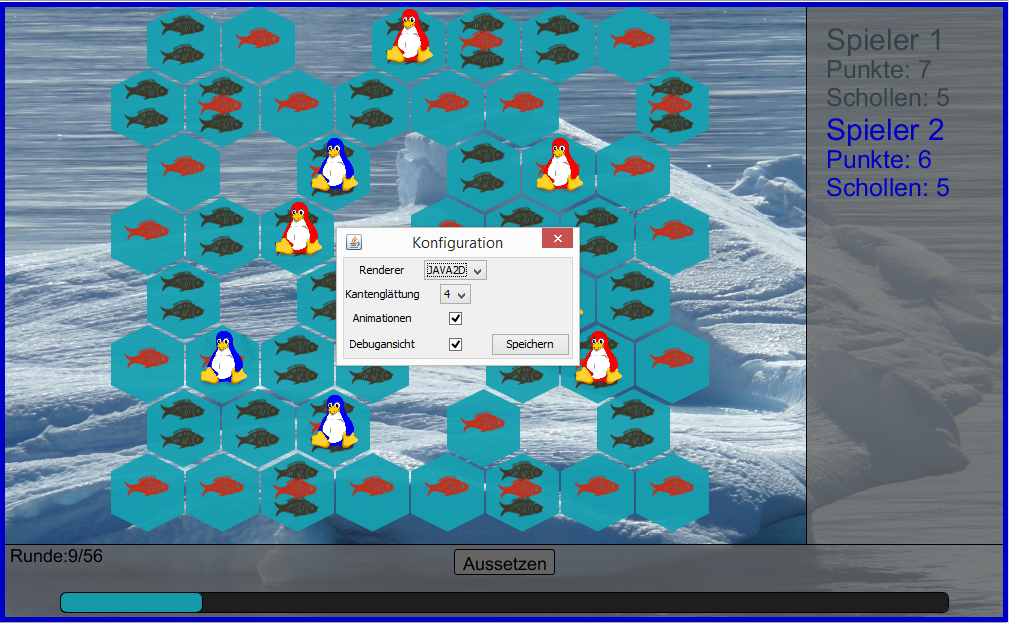
\includegraphics[scale=0.4]{bilder/konfiguration.png}
		\caption{Das Einstellungsmenü}
		\label{fig:Configuration}
	\end{figure}
	
	Ein Einstellungsmenü mit Darstellungsoptionen lässt
sich über die Leertaste anzeigen. Dazu muss das
Spielfeld den Tastaturfokus haben (erforderlichenfalls
vorher Mausklick auf das Spielfeld). Es stehen dort
folgende Einstellungen zur Verfügung: 

\textbf{Kantenglättung} und \textbf{Transparenz} verbessern die Optik des
Spiels, sind aber rechenintensiv. Auf sehr langsamen Rechnern sollten sie daher
deaktiviert werden. \textbf{Hintergrundbild} ist zwar weniger rechenintensiv,
kann aber auch aus Gründen der Übersichtlichkeit deaktiviert werden.\\
\textbf{Animationen} legt fest, ob die Bewegungen der Spielsteine in
Wiederholungen und bei Computerspielern animiert werden sollen.\\
Die \textbf{Debugansicht} verkleinert die Punkteanzeige in der Seitenleiste
etwas und zeigt unterhalb Debug-Hilfestellungen zu einzelnen Zügen an. Diese
Hilfestellungen sind Texte, die ein Spielclient einem Zug beifügen kann, den er
an den Spielserver sendet.
	
\end{document}
